\section{Identification \& Authentication}
\label{sec:ianda}

\subsection*{Einführung}

``Identification \& Authentication'' (I\&A) fasst folgende zwei Schritte zusammen:

\begin{enumerate}
	\item Feststellen der Identität eines Subjektes sowie Verbindung zu einer im System abgelegten ID herstellen (Identification)
	\item Mittels einem Authenticator\footnote{Als Authenticator gilt z.B. ein Passwort, Hardwaretoken, Streichliste usw.} prüfen, ob Subjekt wirklich für die ermittelte ID berechtigt ist (Authentication)
\end{enumerate}

Für dieses grundlegende Schema gibt es zwei verschiedene Varianten:

\begin{enumerate}
	\item Ein Subjekt wird mit einer eindeutigen Identität in Verbindung gebracht (Individual I\&A)
	\item Ein Subjekt wird lediglich auf die Zugehörigkeit zu einer Gruppe geprüft (Group I\&A)\\
	Beispiel: Wache prüft jede Person an der Pforto, ob er einen Mitarbeiterbadge bei sich trägt.
\end{enumerate}

Um I\&A einsetzen zu können ist eine Reihe weiterer (aktiver und passiver) Komponenten nötig:
\begin{itemize}
	\item \emph{Subjektregistrierung}: Ein Subjekt muss initial registriert werden, damit es später wieder identifizert und authentifiziert werden kann
	\item \emph{Sessionmanagement}: Schlagwort Single-Sign-On
	\item \emph{Gesicherte Systemkomponenten, ``Using function''}: Komponenten, welche I\&A aufrufen und dessen Output verwenden (z.B. Patterns aus dem Kapitel \ref{sec:accesscontrolmodels})
\end{itemize}

\begin{figure}[H]
	\centering
	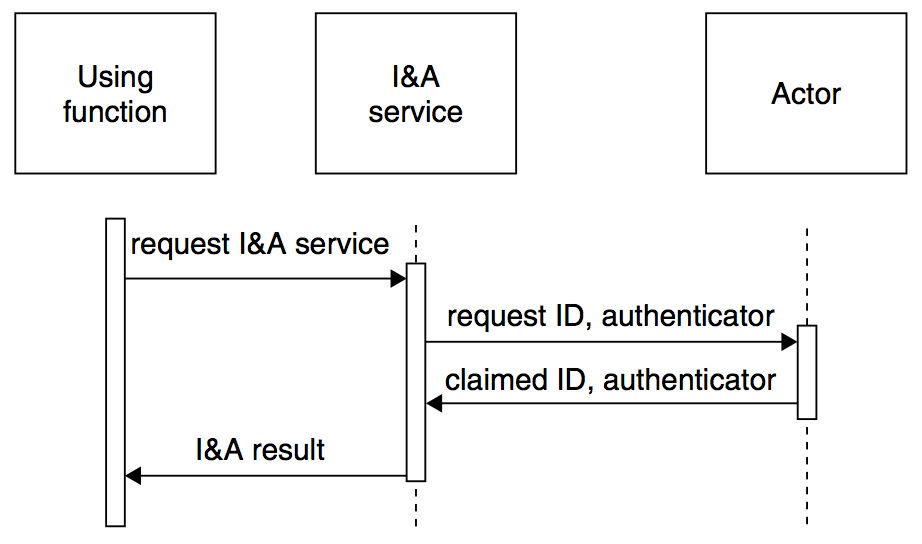
\includegraphics[width=8cm]{content/security/identification-and-authentication/using-functions.png}
	\caption{Generischer Ansatz von I\&A ``Using functions'' \cite{SecPatterns06}}
\end{figure}

\subsection*{Mögliche Prüfungsfragen}
\begin{itemize}
	\item \emph{Was ist ein Authenticator?}\\
	Nachdem ein Subjekt mit einer im System abgelegten Identität in verbindung gebracht wurde, wird der Authenticator verwendet, um sicherzustellen, dass das Subjekt auch wirklich das Subjekt ist, für welches es sicht ausgibt.\\
	Beispiel: Nach Eingabe des Benutzernamens wird das Passwort als Authenticator verwendet.

	\item \emph{Welche grundlegenden Typen von I\&A unterscheidet man?}\\
	Individual und Group Identification \& Authentication
\end{itemize}

\subsection{I\&A Requirements}
\label{sec:ianda-requriements}

Muss ein I\&A Service etabliert werden, hilft das I\&A Requirements Pattern mit seinen generischen Requirementsvorlagen bei der Analyse eines bestehenden oder zu konzipierenden Systems.

Dabei werden nicht nur sicherheitsrelevante Faktoren berücksichtigt. Aspekte wie Kosteneffektivität oder Benutzerzufriedenheit und -akzeptanz fliessen ebenso in die Analyse mitein.

\subsection*{Kontext}
Eine Organisation oder ein Projekt konzipiert die Verwendung von I\&A. Das Pattern unterstützt die Analyse jeglicher Situationen, in welchen sowohl Identification als auch Authorization notwendig ist.

\subsection*{Problem}
Der Natur nach können Anforderungen oftmals im Konflikt zueinander stehen. Insbesondere im Bereich der I\&A können hohe Sicherheitsanforderungen nicht mit dem tiefen Projektbudget vereinbar sein.

Wie können nun aber eben diese Anforderungen auf die aktuelle Situation angepasst miteinander in Einklang gebracht werden?

\subsection*{Lösung}
Das I\&A Requirements Pattern definiert folgende Vorgehensweise:

\begin{enumerate}
	\item \emph{Requirements Specification}\\
	Generische Requirementsvorlagen im Systemdesign-Prozess aufgreifen und auf eigene Situation anpassen
	\item \emph{Prioritization Process}\\
	Die Menge an angepassten, generischen Requirements wird nun gem. der aktuellen Situation priorisiert
\end{enumerate}

\subsubsection*{Generische Requirementsvorlagen}

\begin{table}[H]
\tablestyle
\tablealtcolored
\begin{tabularx}{\textwidth}{l X}
\tableheadcolor
	\tablehead Anforderung &
	\tablehead Erläuterung \tabularnewline
\tablebody
	Accuratly Detect Imposters &
	Requests von unberechtigten Actors sollen als solche erkannt werden.
	\tabularnewline
	Accuratly Recognize Legitimate Actors &
	Korrekte Requests an den Service sollen auch als solche erkannt werden.
	\tabularnewline
\tableend
\end{tabularx}
\caption{I\&A Requirements: Funktionale Anforderungen}
\end{table}

Die beiden funktionalen Anforderungen stehen praktisch immer in gegenseitiger Wechselwirkung: Werden mehr Requests als \emph{Falsch} klassifiziert, erwischt man automatisch auch mehr Requests, welche eigentlich \emph{Richtig} gewesen wären.

\begin{table}[H]
\tablestyle
\tablealtcolored
\begin{tabularx}{\textwidth}{l X}
\tableheadcolor
	\tablehead Anforderung &
	\tablehead Erläuterung \tabularnewline
\tablebody
	Minimize Mismatch with user Characteristics &
	Unterschiedliche Wissensstände, Umgebungseinflüsse (Standort ...) usw. von Actors sollen zu so wenigen wie möglichen Fehlinterpretationen von Service Requests führen.
	\tabularnewline
	Minimize Time and Effort to Use &
	Bspw. Zeitaufwand für mehrmaliges eintippen des Passworts soll verhindert werden
	\tabularnewline
	Minimize Risks to User Safety &
	Beispiel: Retina Scanner muss mit Gasmaske funktionieren; dies steht im Konflikt mit der Genauigkeit der Requesterkennung
	\tabularnewline
	Minimize Costs of Per-user Setup &
	\tabularnewline
	Minimize Changes Needed to\\Existing System Infrastr. &
	Soll der I\&A Service in ein bestehendes System integriert werden, sollen die anfallenden Änderungen in der bestehenden Infrastruktur ggf. minimiert werden
	\tabularnewline
	Minimize Costs of Maintainance,\\Management \& Overhead &
	\tabularnewline
	Protect I\&A Service and Assets &
	Wie wichtig ist der Schutz des I\&A Services und er zu schützenden Objekte?
	\tabularnewline
\tableend
\end{tabularx}
\caption{I\&A Requirements: Nichtfunktionale Anforderungen}
\end{table}

\subsubsection*{Analogie: Anlagestrategie im Finanzsektor}
Es können nie alle Anforderung gleich gut abgedeckt werden. Wie bei einer Anlagestrategie (Dreieck \emph{Liquidität, Sicherheit, Rentabilität}) müssen alle Anforderungen analysiert und auf die eigene Situation/Präferenzen zugeschnitten werden.

\subsection*{Vorteile}
\begin{itemize}
	\item Eine ausführliche Domain- und Anforderungsanalyse wird gefördert.
	\item Die vorliegenden Requirementsvorlagen fördern die ausführliche Auseinandersetzung mit den verschiedensten Einflüsse auf I\&A.
	\item Als angenehmen Nebeneffekt erhält man eine Umfangreiche Dokumentation über die I\&A Aspekte des Systems.
\end{itemize}

\subsection*{Nachteile}
\begin{itemize}
	\item Der Aufwand zur Umsetzung dieses Patterns kann tendenziell sehr Resourcenintensiv sein (Anforderungsanalyse, Priorisierung etc. etc.)
	\item Die vielen Ausprägungen der einzelnen Anforderungen können leicht in einem Over-Engineering enden. Diese Gefahr kann jedoch durch pragmatische Herangehensweise (Verwendung als Guidelines) minimiert werden
	\item Da eine umfangreiche Dokumentation als Resultat des Patterns ensteht, besteht natürlich auch die Gefahr, dass diese im Laufe der Zeit nicht mehr aktualisiert wird.
\end{itemize}

\subsection*{Mögliche Prüfungsfragen}
\begin{itemize}
	\item \emph{Gibt es ein I\&A Patentrezept?}\\
	Nein. Jedes System kommt mit seinen eigenen, spezifischen Anforderungen an I\&A. Aus diesem Grund kann und sollte das I\&A Requirements Pattern nur als Guideline/Vorlage zu eigenen spezifischen Implementierungen verwendet werden.
\end{itemize}